\documentclass[12pt, a4paper]{article}

\usepackage{graphicx, caption, subcaption, float}     % Figures
\usepackage{minted, xcolor}    % Code
\usepackage{hyperref}    % Links

\renewcommand{\thesubsection}{\alph{subsection}}

\definecolor{cbg}{rgb}{0.95, 0.95, 0.95}

\begin{document}

\begin{titlepage}
\center
\textsc{\LARGE Nanyang Technological University}\\[20mm]
\textsc{\Large CZ4003 Computer Vision}\\[40mm]
\rule{\linewidth}{0.3mm}\\[8mm]
{\huge\bfseries Lab 1}\\[4mm]
\rule{\linewidth}{0.3mm}\\[25mm]
\begin{flushright} \large
Onno \textsc{Eberhard}\\
N1804715F
\end{flushright}~\\[45mm]
{\large \today}
\vfill % Fill the rest of the page with whitespace
\end{titlepage}

\tableofcontents
\newpage

\section{Contrast Stretching}
\subsection{Load image and transform to greyscale}
Input:
\begin{minted}[bgcolor=cbg, fontsize=\footnotesize, mathescape]{octave}
img = imread('mrt-train.jpg');
whos img
\end{minted}
Output:
\begin{minted}[bgcolor=cbg, fontsize=\footnotesize, mathescape]{text}
Name        Size                Bytes  Class    Attributes

img       320x443x3            425280  uint8           
\end{minted}
Input:
\begin{minted}[bgcolor=cbg, fontsize=\footnotesize, mathescape]{octave}
img = rgb2gray(img);
whos img
\end{minted}
Output:
\begin{minted}[bgcolor=cbg, fontsize=\footnotesize, mathescape]{text}
Name        Size              Bytes  Class    Attributes

img       320x443            141760  uint8       
\end{minted}
\subsection{Display the image}
Input:
\begin{minted}[bgcolor=cbg, fontsize=\footnotesize, mathescape]{octave}
figure
imshow(img)
\end{minted}
\newpage
Output:
\begin{figure}[H]
	\centering
	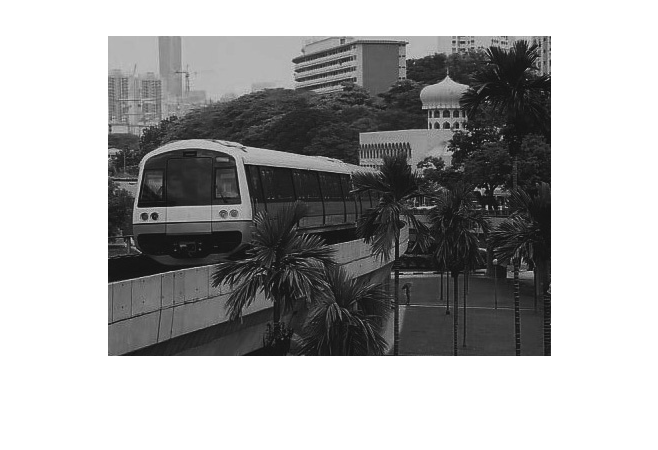
\includegraphics[width=\textwidth]{fig1.png}
\end{figure}
\vspace{-10mm}
\subsection{Find minimum and maximum intensity values}
The values should ideally be 0 and 255 respectively.\\
Input:
\begin{minted}[bgcolor=cbg, fontsize=\footnotesize, mathescape]{octave}
r_min = double(min(img(:)))    % Convert to double for later use
r_max = double(max(img(:)))
\end{minted}
Output:
\begin{minted}[bgcolor=cbg, fontsize=\footnotesize, mathescape]{text}
r_min = 13
r_max = 204
\end{minted}
\newpage
\subsection{Contrast stretching}
Input:
\begin{minted}[bgcolor=cbg, fontsize=\footnotesize, mathescape]{octave}
img = uint8(255 * (double(img) - r_min) / (r_max - r_min));
assert(min(img(:)) == 0 && max(img(:)) == 255)    % Check if it worked
\end{minted}
The assertion would throw an error if the contrast stretching had failed. Because there is no output, everything worked as expected.
\subsection{Display the enhanced image}
Input:
\begin{minted}[bgcolor=cbg, fontsize=\footnotesize, mathescape]{octave}
figure
imshow(img)
\end{minted}
Output:
\begin{figure}[ht]
	\centering
	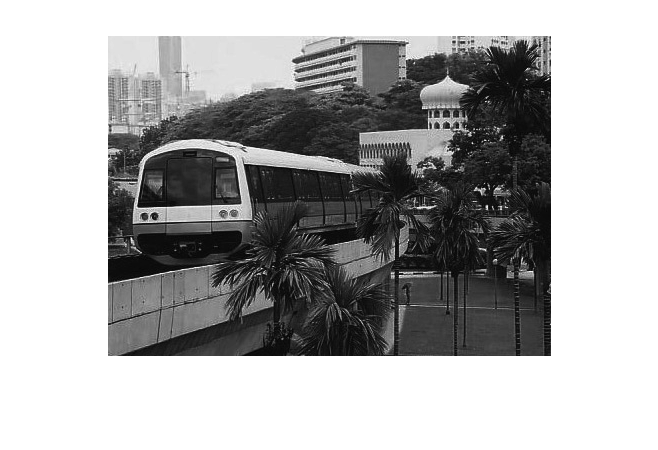
\includegraphics[width=\textwidth]{fig2.png}
\end{figure}

\section{Histogram Equalization}
\subsection{Intensity histograms}
Input:
\begin{minted}[bgcolor=cbg, fontsize=\footnotesize, mathescape]{octave}
figure
imhist(img, 10)
figure
imhist(img, 256)
\end{minted}
Output:
\begin{figure}[H]
    \centering %use either centering or hfill (between images)
    \begin{subfigure}[b]{0.7\textwidth}
        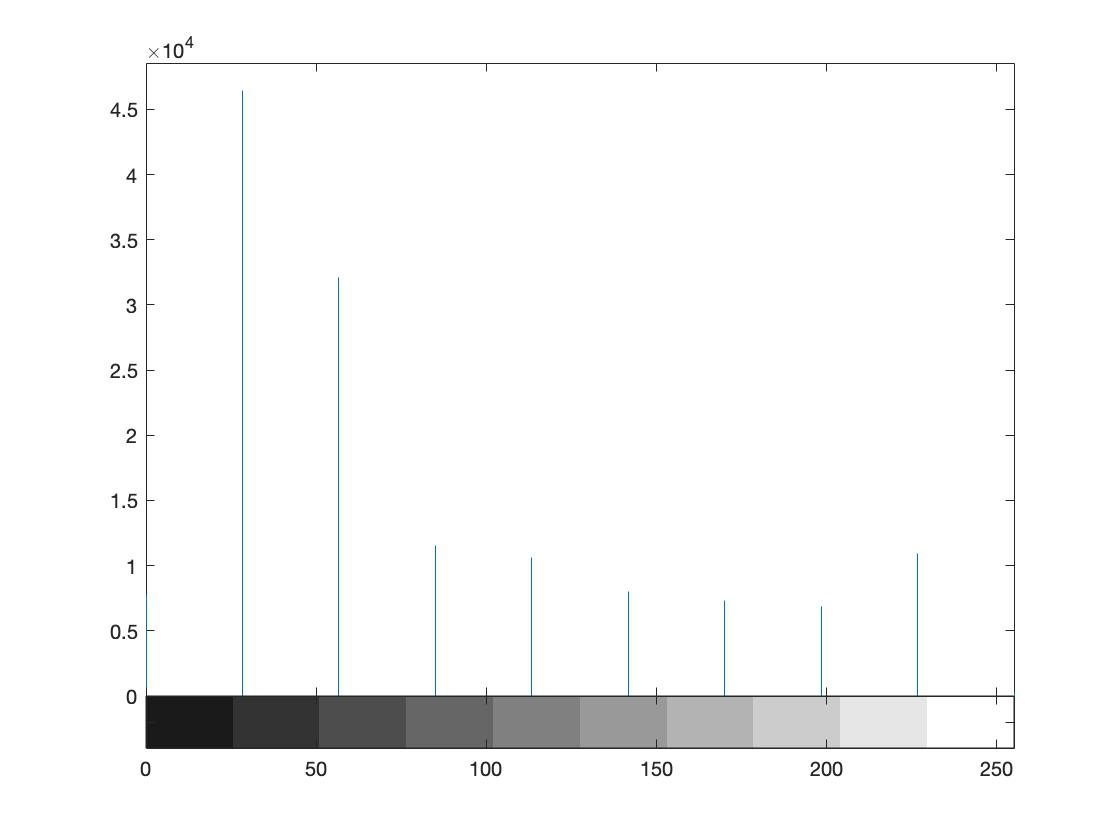
\includegraphics[width=\textwidth]{fig3.png}
        %\caption{Flower one.}
        %\label{fig:f1}
    \end{subfigure}
    %\hfill
    \begin{subfigure}[b]{0.7\textwidth}
        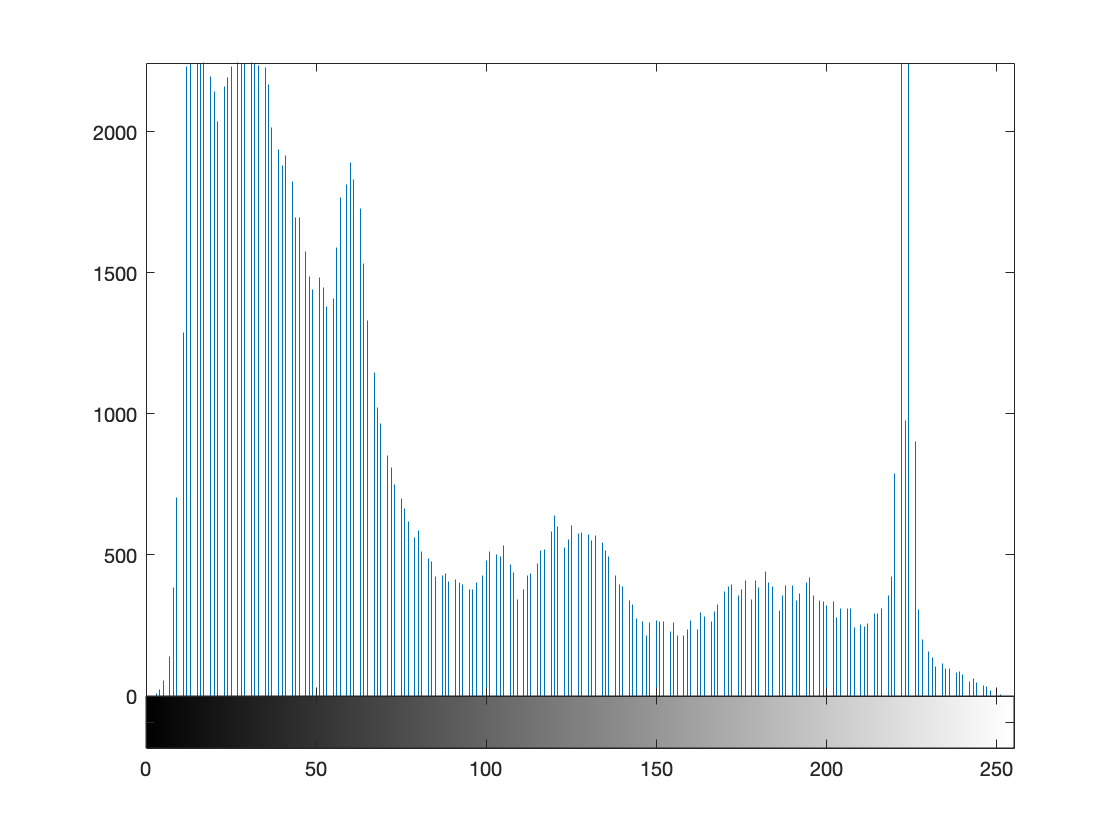
\includegraphics[width=\textwidth]{fig4.png}
        %\caption{Flower two.}
        %\label{fig:f2}
    \end{subfigure}
    %\caption{My flowers.}
\end{figure}
~\\
The first histogram shows much less detail, it divides the 256 intensity levels into 10, making every bin hold on average 256/10 = 25.6 times as many pixels as in the second histogram, where all 256 intensity levels get their own bin. An example of detail that gets lost in the first histogram is the spike at the intensity levels between 220 and 226.
\subsection{Histogram equalization}
Input:
\begin{minted}[bgcolor=cbg, fontsize=\footnotesize, mathescape]{octave}
img_eq = histeq(img, 256);    % 256 discrete intensity levels -> N=256
figure
imhist(img_eq, 10)
figure
imhist(img_eq, 256)
\end{minted}
Output:
\begin{figure}[h]
    \centering
    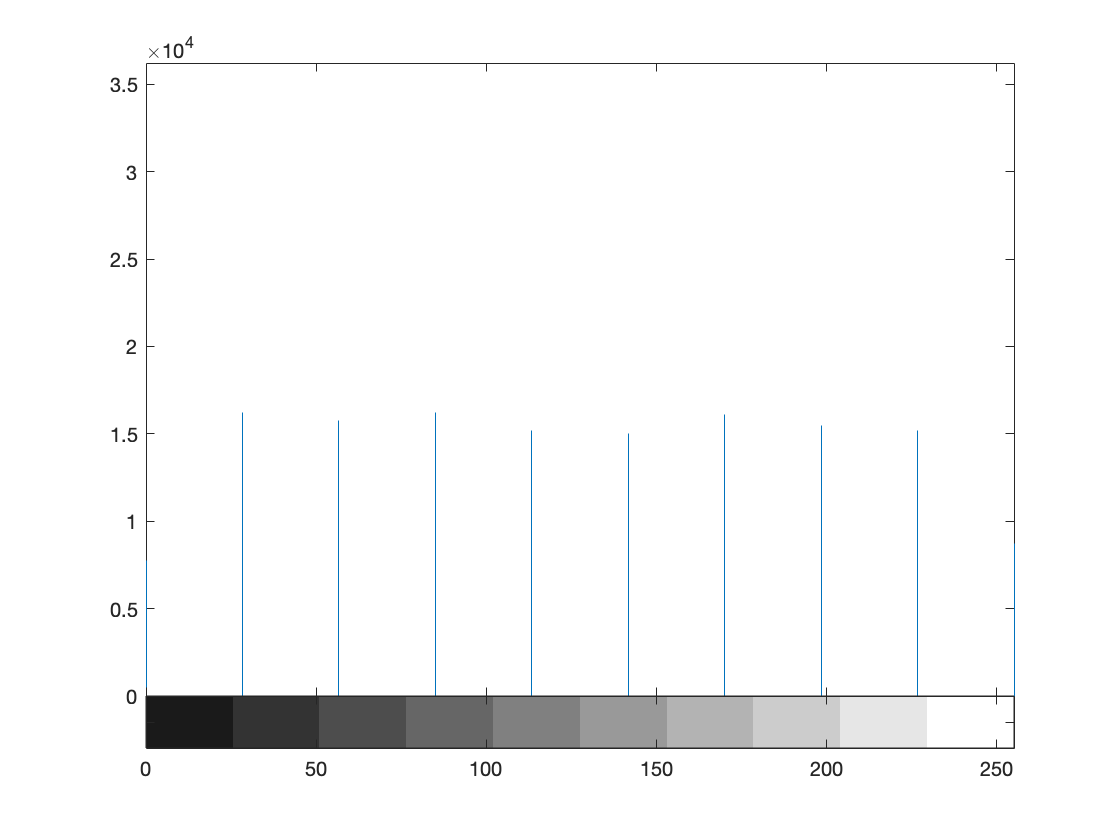
\includegraphics[width=0.7\textwidth]{fig5.png}
\end{figure}
\begin{figure}[H]
    \centering
    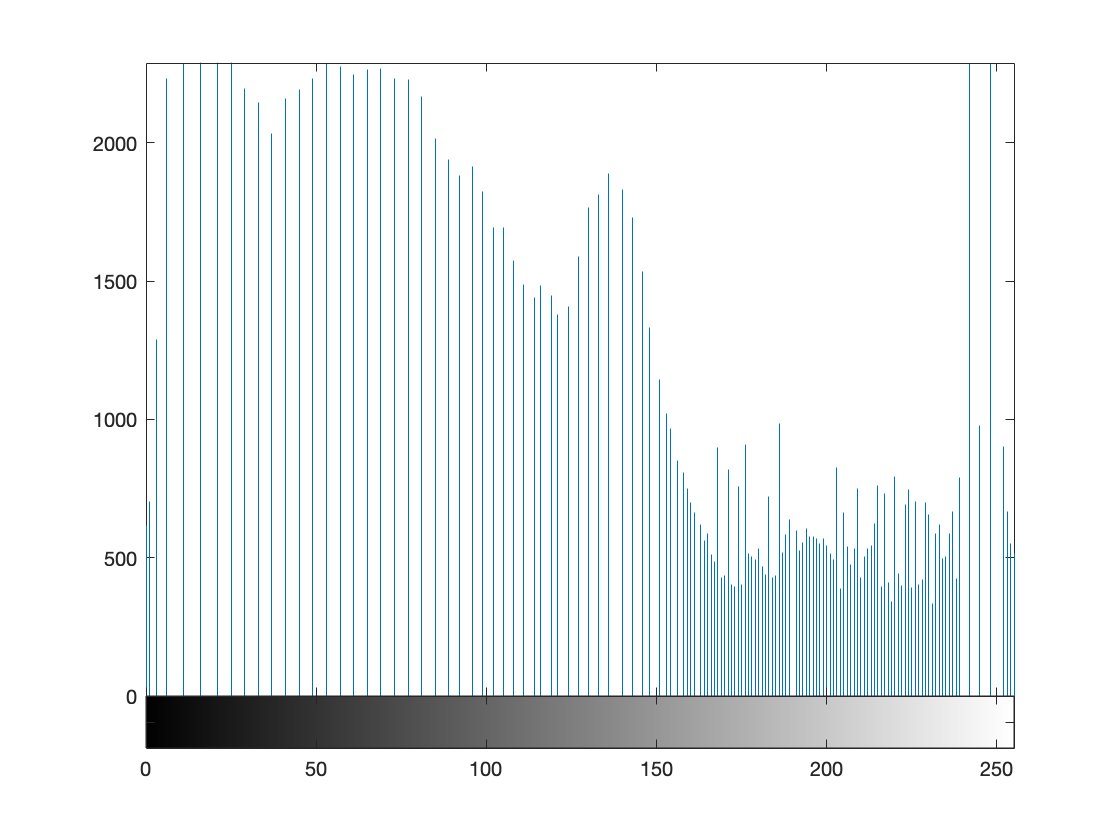
\includegraphics[width=0.7\textwidth]{fig6.png}
\end{figure}
~\\
The histograms are equalized, this is very obvious in the first figure, but less so in the second. The second histogram shows that there are now many intensity levels that do not hold any pixels. This is because of how the histogram equalization algorithm works. The density in the second histogram is very consistent, with some regions having a few, highly packed intensity values, and others having many, but less packed ones.
\subsection{Repeat histogram equalization}
Input:
\begin{minted}[bgcolor=cbg, fontsize=\footnotesize, mathescape]{octave}
img_eq2 = histeq(img_eq, 256);
figure
imhist(img_eq2, 10)
figure
imhist(img_eq2, 256)
\end{minted}
\newpage
Output:
\begin{figure}[H]
    \centering
    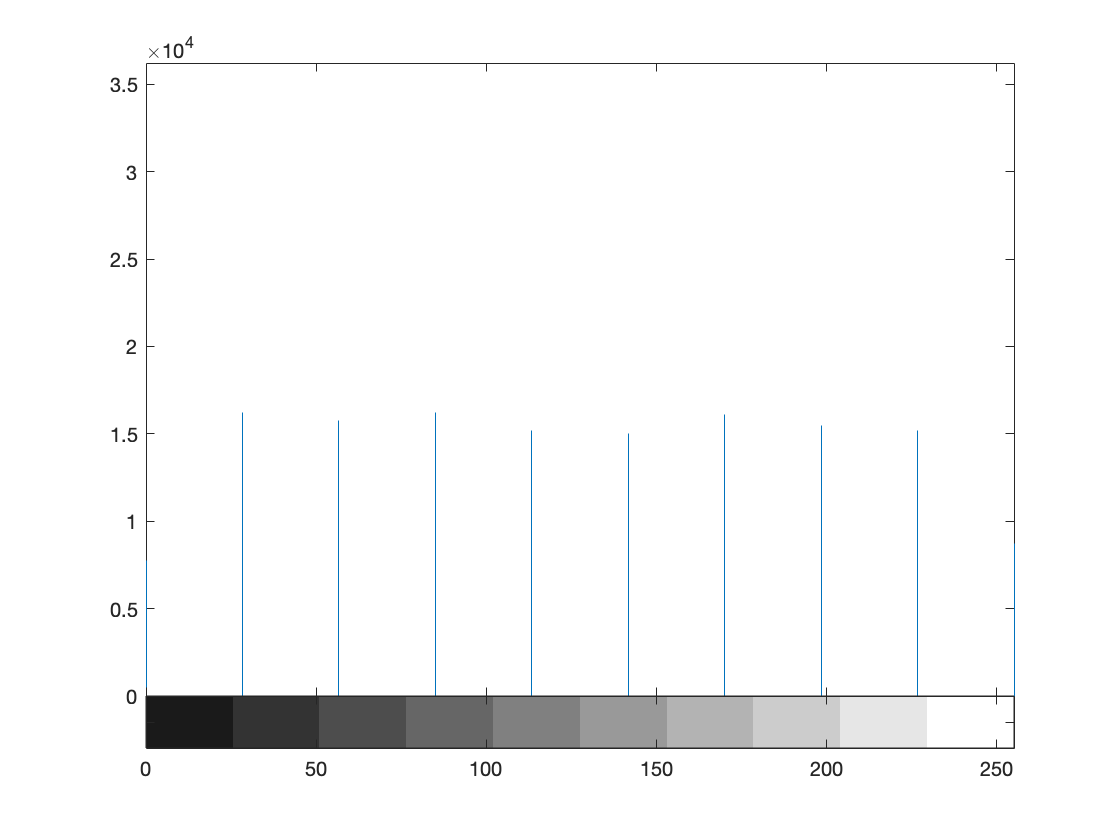
\includegraphics[width=0.7\textwidth]{fig5.png}
\end{figure}
\begin{figure}[H]
    \centering
    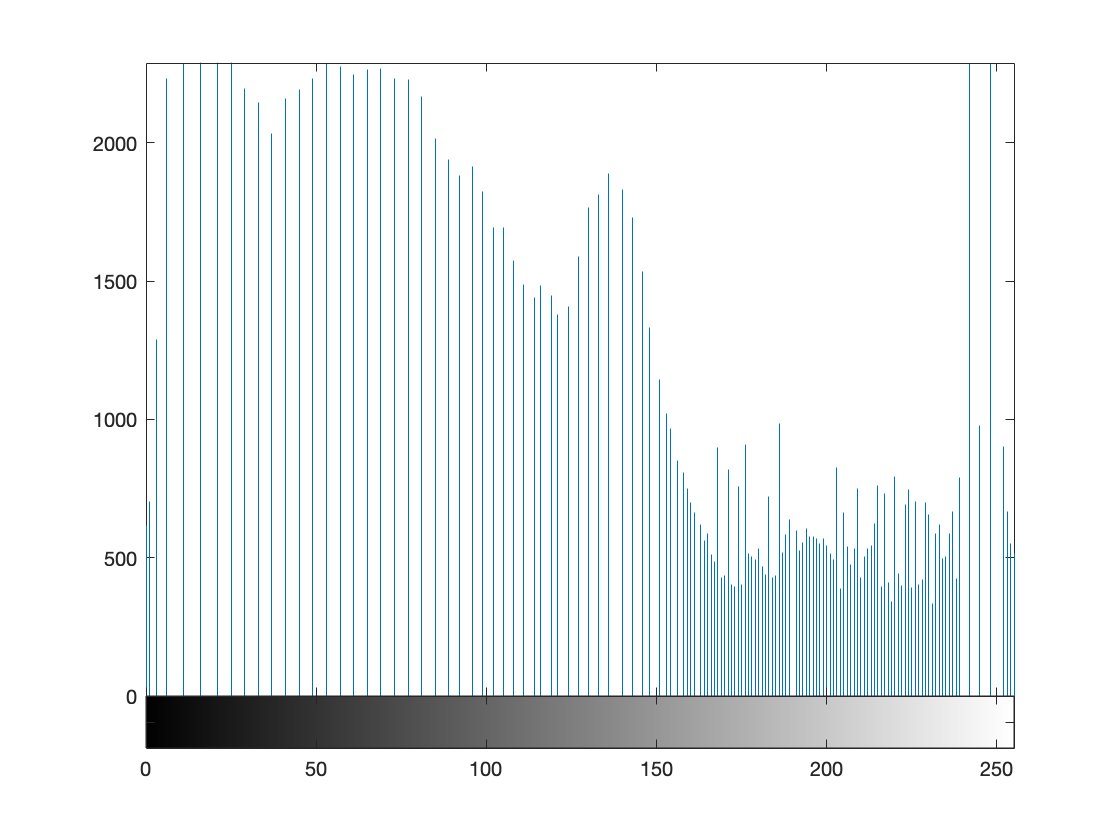
\includegraphics[width=0.7\textwidth]{fig6.png}
\end{figure}
~\\
The histograms do not become more uniform. In history equalization, repeated application does not lead to better results. This is because bins will only be combined, and never separated. The algorithm does not necessarily optimize towards a completely flat histogram, this will only be the case in very few special cases.

\section{Linear Spatial Filtering}
\subsection{Generate the filters}
Input:
\begin{minted}[bgcolor=cbg, fontsize=\footnotesize, mathescape]{octave}
h = @(sigma, x, y) 1 / (2 * pi * sigma^2) ...
                   * exp(-(x.^2 + y.^2) / (2 * sigma^2));
[x, y] = meshgrid(-2:2);
h1 = h(1, x, y);
h1 = h1 / sum(h1(:));
h2 = h(2, x, y);
h2 = h2 / sum(h2(:));

figure
surf(x, y, h1)    % Mesh looked more boring
figure
surf(x, y, h2)
\end{minted}
Output:
\begin{figure}[H]
    \centering %use either centering or hfill (between images)
    \begin{subfigure}[b]{0.45\textwidth}
        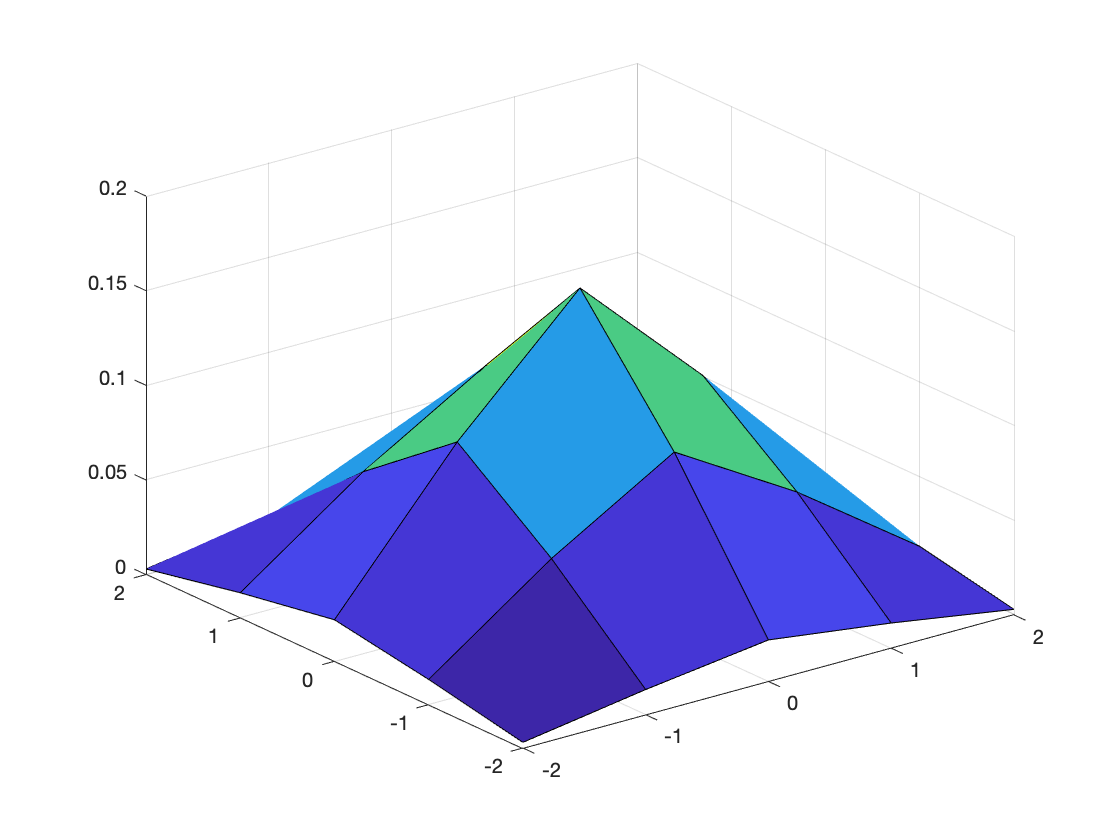
\includegraphics[width=\textwidth]{fig9.png}
        %\caption{Flower one.}
        %\label{fig:f1}
    \end{subfigure}
    %\hfill
    \begin{subfigure}[b]{0.45\textwidth}
        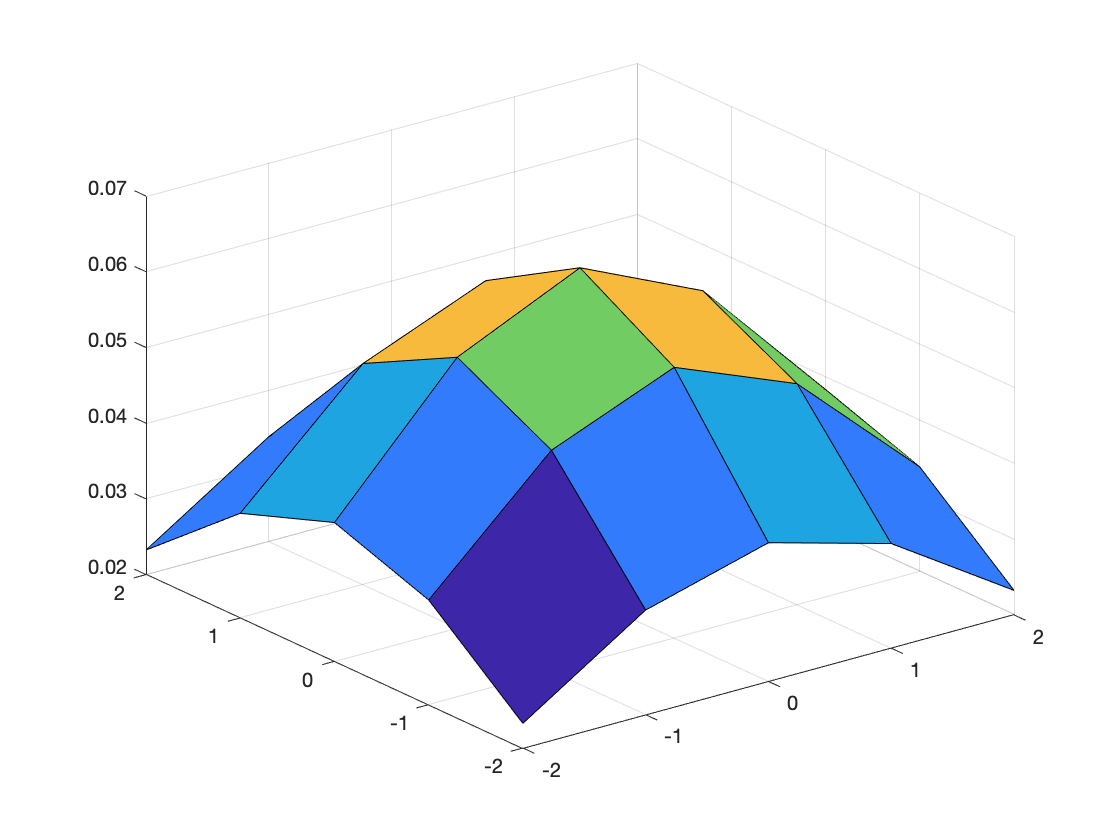
\includegraphics[width=\textwidth]{fig10.png}
        %\caption{Flower two.}
        %\label{fig:f2}
    \end{subfigure}
    %\caption{My flowers.}
\end{figure}
\subsection{Load and view image}
\begin{minted}[bgcolor=cbg, fontsize=\footnotesize, mathescape]{octave}
img = imread('ntugn.jpg');
figure
imshow(img)
\end{minted}
\begin{figure}[H]
    \centering
    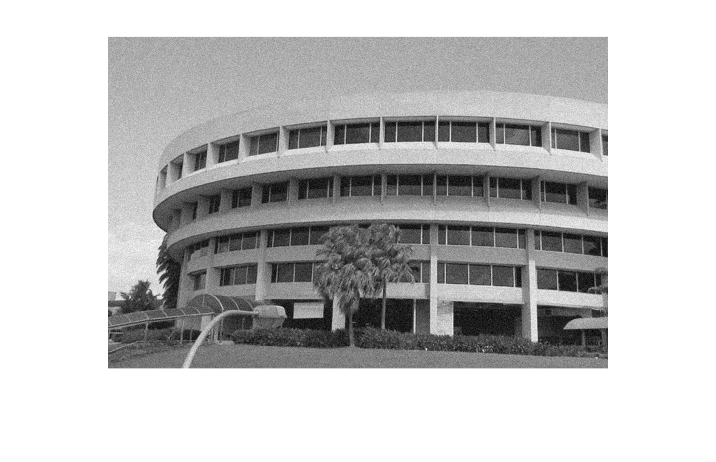
\includegraphics[width=0.7\textwidth]{fig11.png}
\end{figure}
\subsection{Filtering the images}
Input:
\begin{minted}[bgcolor=cbg, fontsize=\footnotesize, mathescape]{octave}
img_h1 = uint8(conv2(img, h1));
figure
imshow(img_h1)

img_h2 = uint8(conv2(img, h2));
figure
imshow(img_h2)
\end{minted}
Output:
\begin{figure}[H]
    \centering
    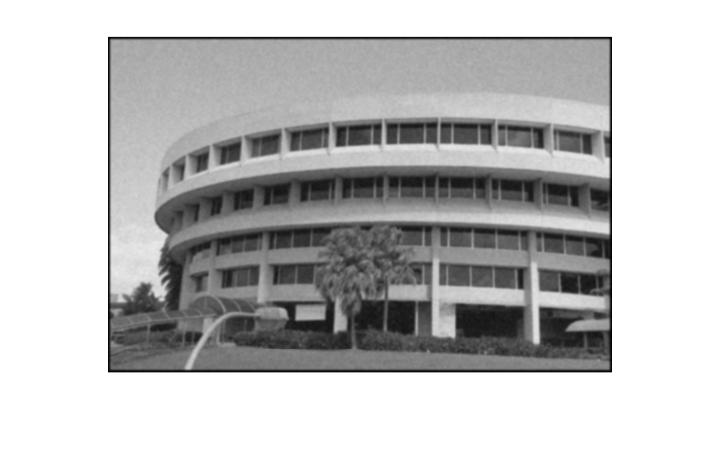
\includegraphics[width=0.7\textwidth]{fig12.png}
\end{figure}
\begin{figure}[H]
    \centering
    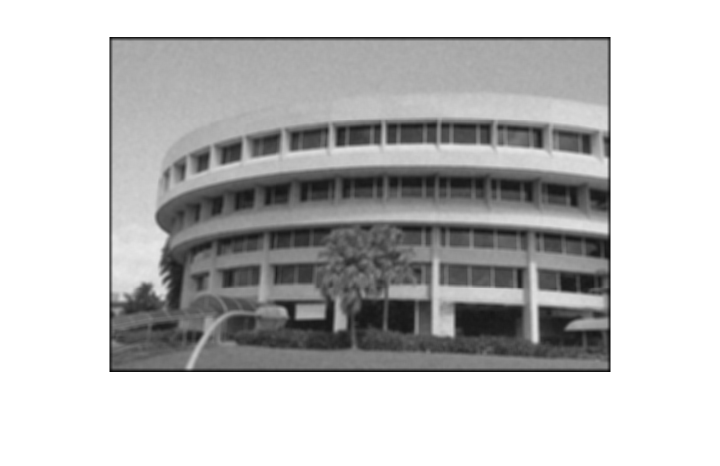
\includegraphics[width=0.7\textwidth]{fig13.png}
\end{figure}
~\\
The filters are not very effective at removing the noise, it is still clearly visible in both filtered images. Both filters do however make the image more blurred, the second filter (higher standard deviation) more so than the first one. The second filter is also better at removing the noise, but the price payed in blur is probably too high to use the filter in this context.

\subsection{Speckle noise}
Input:
\begin{minted}[bgcolor=cbg, fontsize=\footnotesize, mathescape]{octave}
img = imread('ntusp.jpg');
figure
imshow(img)
\end{minted}
Output:
\begin{figure}[H]
    \centering
    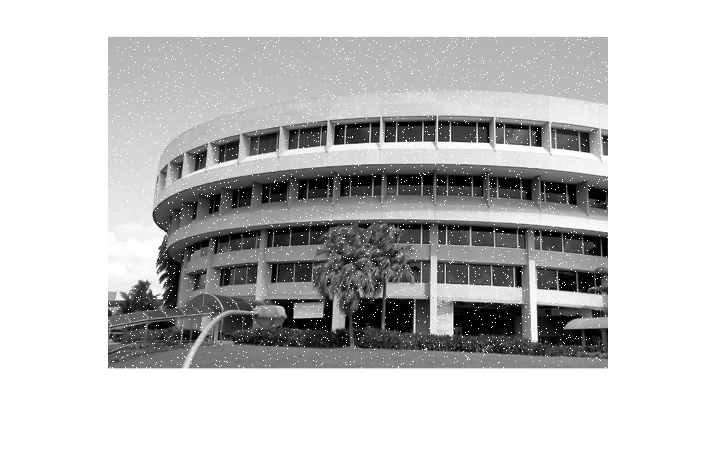
\includegraphics[width=0.7\textwidth]{fig14.png}
\end{figure}

\subsection{Filtering speckle noise}
Input:
\begin{minted}[bgcolor=cbg, fontsize=\footnotesize, mathescape]{octave}
img_h1 = uint8(conv2(img, h1));
figure
imshow(img_h1)

img_h2 = uint8(conv2(img, h2));
figure
imshow(img_h2)
\end{minted}
Output:
\begin{figure}[H]
    \centering
    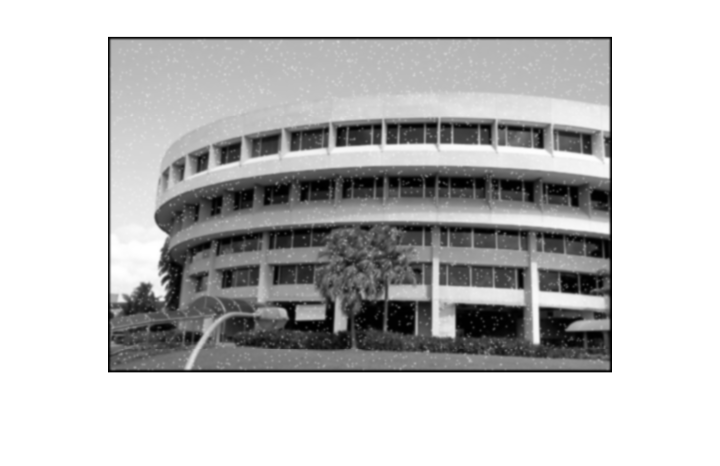
\includegraphics[width=0.7\textwidth]{fig15.png}
\end{figure}
\begin{figure}[H]
    \centering
    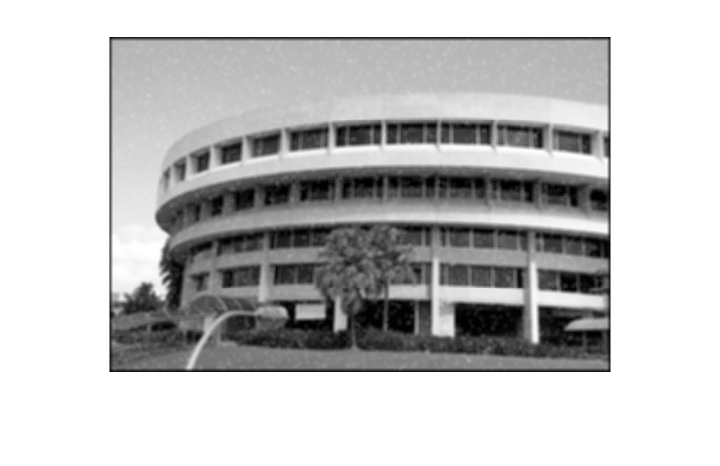
\includegraphics[width=0.7\textwidth]{fig16.png}
\end{figure}
~\\
The filters are better at handling gaussian noise than speckle noise. For speckle noise a median filter is better suited.

\section{Median Filtering}
\subsection{Median filtering gaussian noise}
Input:
\begin{minted}[bgcolor=cbg, fontsize=\footnotesize, mathescape]{octave}
img = imread('ntugn.jpg');

img_h1 = uint8(medfilt2(img, [3, 3]));
figure
imshow(img_h1)

img_h2 = uint8(medfilt2(img, [5, 5]));
figure
imshow(img_h2)
\end{minted}
Output:
\begin{figure}[H]
    \centering
    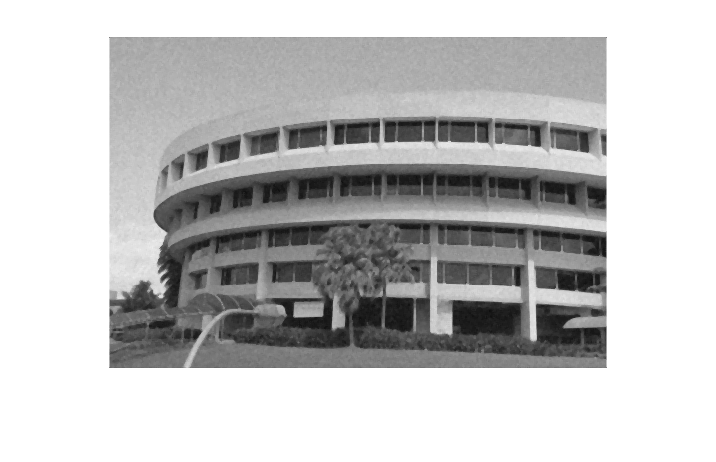
\includegraphics[width=0.7\textwidth]{fig17.png}
\end{figure}
\begin{figure}[H]
    \centering
    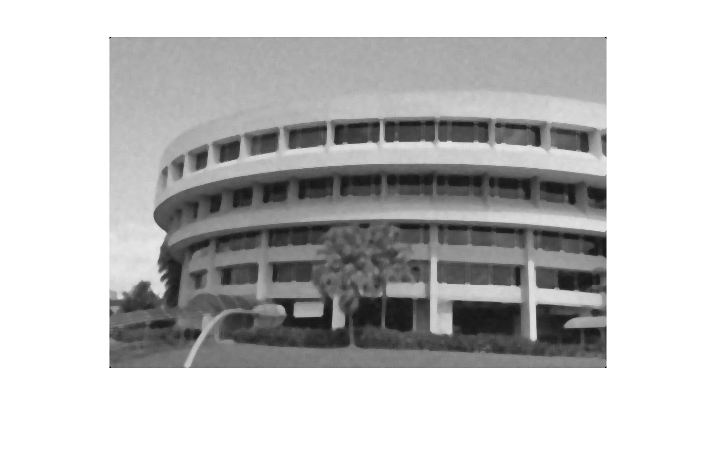
\includegraphics[width=0.7\textwidth]{fig18.png}
\end{figure}
~\\
Gaussian filtering does a better job of filtering out gaussian noise. Median filtering often just amplifies the gaussian noise because in a given region, a noisy pixel might well have the median intensity. This results in an image that is not blurred, like with gaussian filtering, but that looks oddly ``flat'', like it has a lower resolution.
\subsection{Median filtering speckle noise}
Input:
\begin{minted}[bgcolor=cbg, fontsize=\footnotesize, mathescape]{octave}
img = imread('ntusp.jpg');

img_h1 = uint8(medfilt2(img, [3, 3]));
figure
imshow(img_h1)

img_h2 = uint8(medfilt2(img, [5, 5]));
figure
imshow(img_h2)
\end{minted}
\newpage
Output:
\begin{figure}[H]
    \centering
    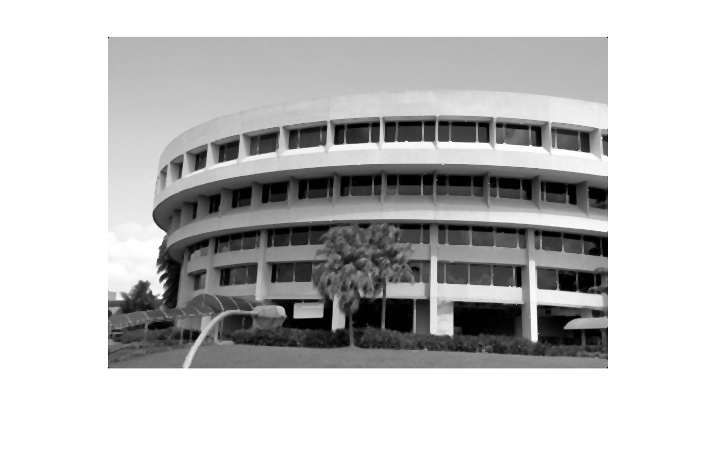
\includegraphics[width=0.7\textwidth]{fig19.png}
\end{figure}
\begin{figure}[H]
    \centering
    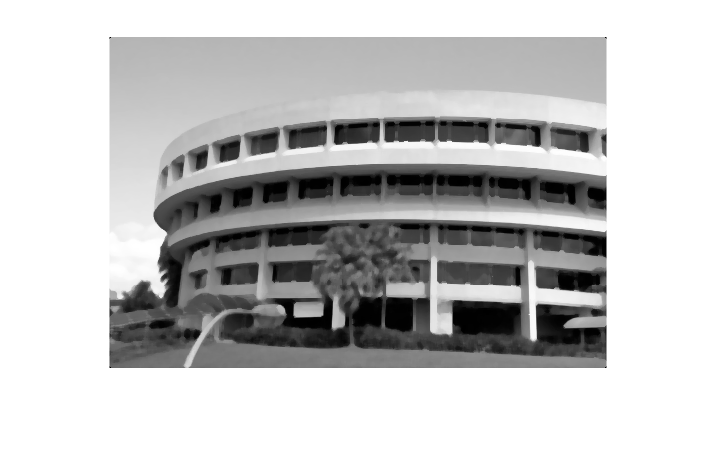
\includegraphics[width=0.7\textwidth]{fig20.png}
\end{figure}
~\\
With speckle noise, median filtering far outshines gaussian filtering. It does not blur the image, and removes the noise completely.
\newpage
\section{Suppressing Noise Interference Patterns}
\subsection{Interference patterns}
Input:
\begin{minted}[bgcolor=cbg, fontsize=\footnotesize, mathescape]{octave}
img = imread('pckint.jpg');
figure
imshow(img)
\end{minted}
Output:
\begin{figure}[H]
    \centering
    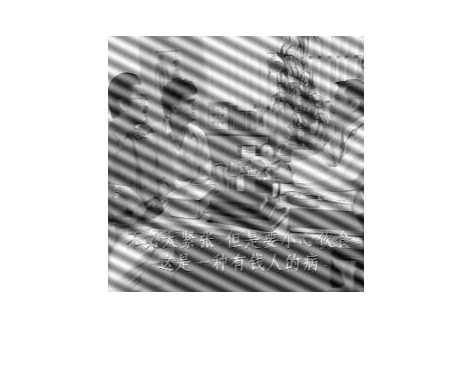
\includegraphics[width=0.7\textwidth]{fig21.png}
\end{figure}

\subsection{Compute Fourier spectrum}
Input:
\begin{minted}[bgcolor=cbg, fontsize=\footnotesize, mathescape]{octave}
ft = fft2(img);
S = abs(ft).^2 / length(img);
figure
imagesc(fftshift(log10(S)))    % Using log10 instead of 10th root
\end{minted}
\newpage
Output:
\\[-12mm]
\begin{figure}[H]
    \centering
    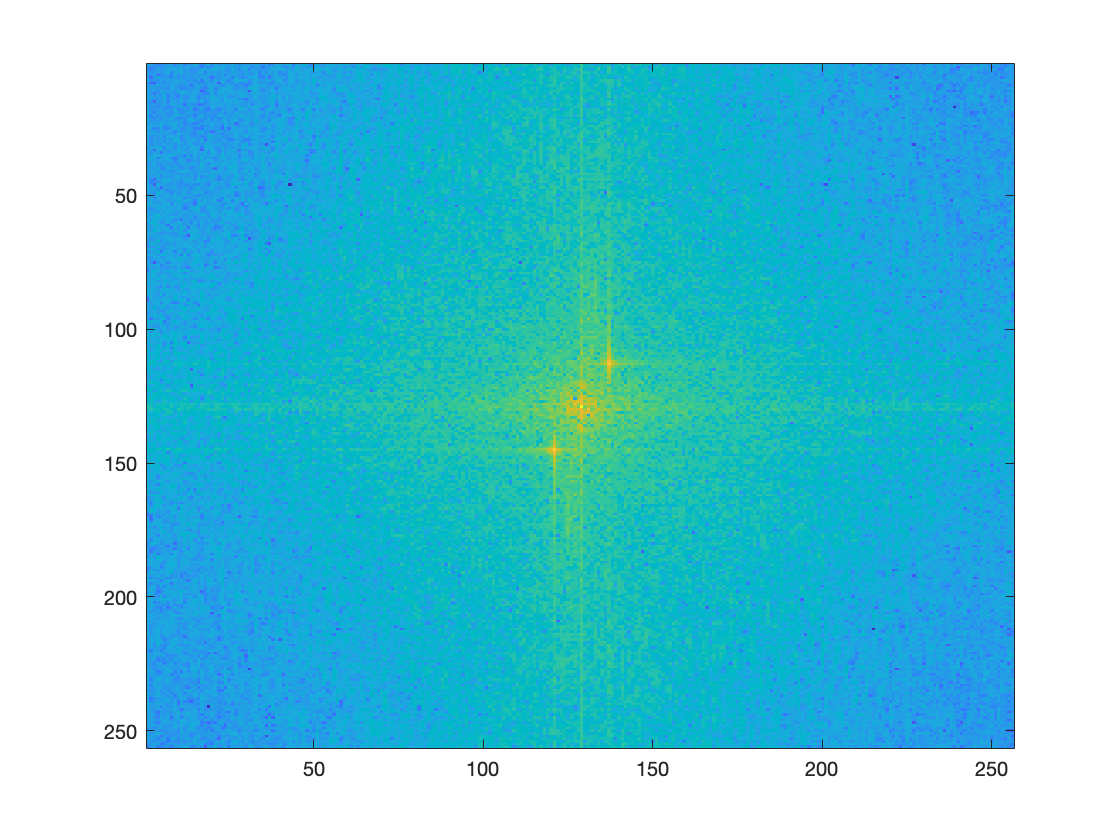
\includegraphics[width=0.7\textwidth]{fig22.png}
\end{figure}
~\\[-15mm]
\subsection{Reading coordinates}
Input:
\begin{minted}[bgcolor=cbg, fontsize=\footnotesize, mathescape]{octave}
figure
imagesc(log10(S))
x1 = 249;
y1 = 17;
x2 = 9;
y2 = 241;
\end{minted}
Output:
\\[-12mm]
\begin{figure}[H]
    \centering
    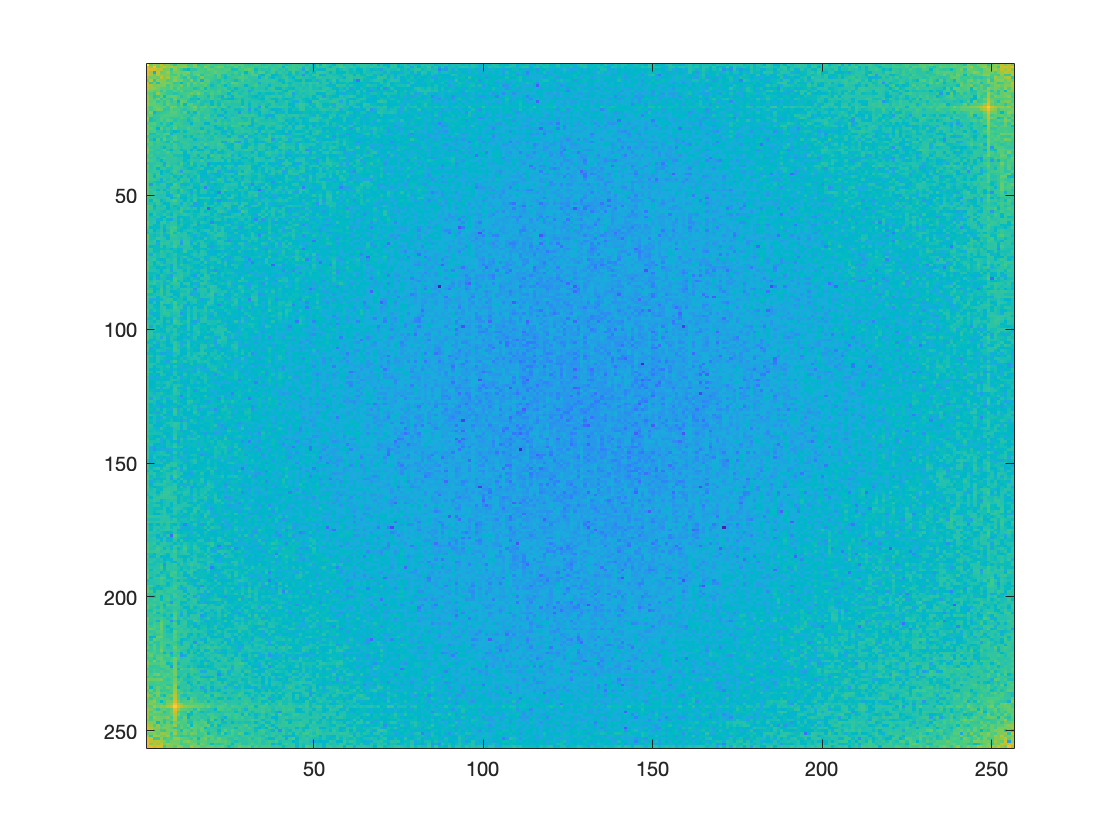
\includegraphics[width=0.7\textwidth]{fig23.png}
\end{figure}

\subsection{Filtering}
Input:
\begin{minted}[bgcolor=cbg, fontsize=\footnotesize, mathescape]{octave}
ft(y1-2 : y1+2, x1-2 : x1+2) = 0;
ft(y2-2 : y2+2, x2-2 : x2+2) = 0;
S = abs(ft).^2 / length(img);
figure
imagesc(fftshift(log10(S)))
\end{minted}
Output:
\begin{figure}[H]
    \centering
    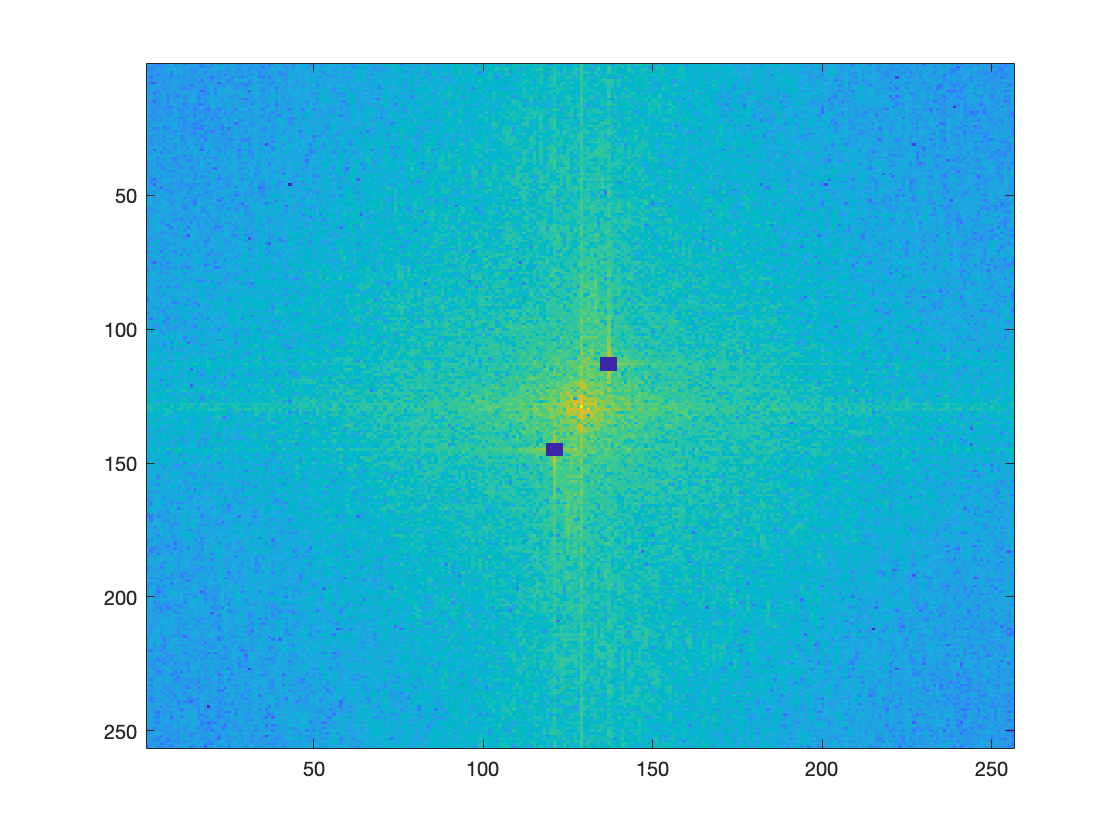
\includegraphics[width=0.7\textwidth]{fig24.png}
\end{figure}

\subsection{Inverse Fourier transform}
Input:
\begin{minted}[bgcolor=cbg, fontsize=\footnotesize, mathescape]{octave}
img = uint8(ifft2(ft));
figure
imshow(img)
\end{minted}
\newpage
Output:
\begin{figure}[H]
    \centering
    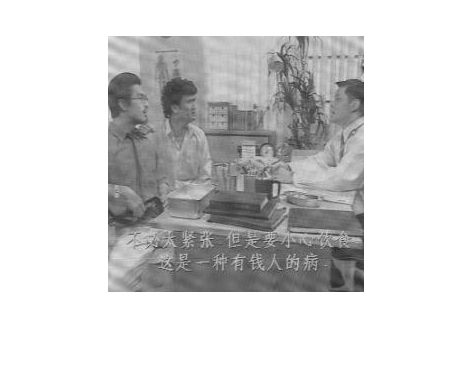
\includegraphics[width=0.7\textwidth]{fig25.png}
\end{figure}
~\\[-15mm]
The resulting image is remarkably better than the original one. The interference is not gone, but at least in the central part almost unnoticeable. In the Fourier spectrum there are lines extending horizontally and vertically from the two blocked interference points. The image may be further enhanced by filtering out those lines as well. Additionally, contrast stretching is necessary because the dynamic range of the image has been reduced substantially by the Fourier filtering.
\\\\
Input:
\begin{minted}[bgcolor=cbg, fontsize=\footnotesize, mathescape]{octave}
% Additional Filtering
ft(y1, :) = 0;
ft(y2, :) = 0;
ft(:, x1) = 0;
ft(:, x2) = 0;
S = abs(ft).^2 / length(img);
figure
imagesc(fftshift(log10(S)))
img = uint8(ifft2(ft));

% Contrast Stretching
r_min = double(min(img(:)));
r_max = double(max(img(:)));
img = uint8(255 * (double(img) - r_min) / (r_max - r_min));

figure
imshow(img)
\end{minted}
Output:
\begin{figure}[H]
    \centering
    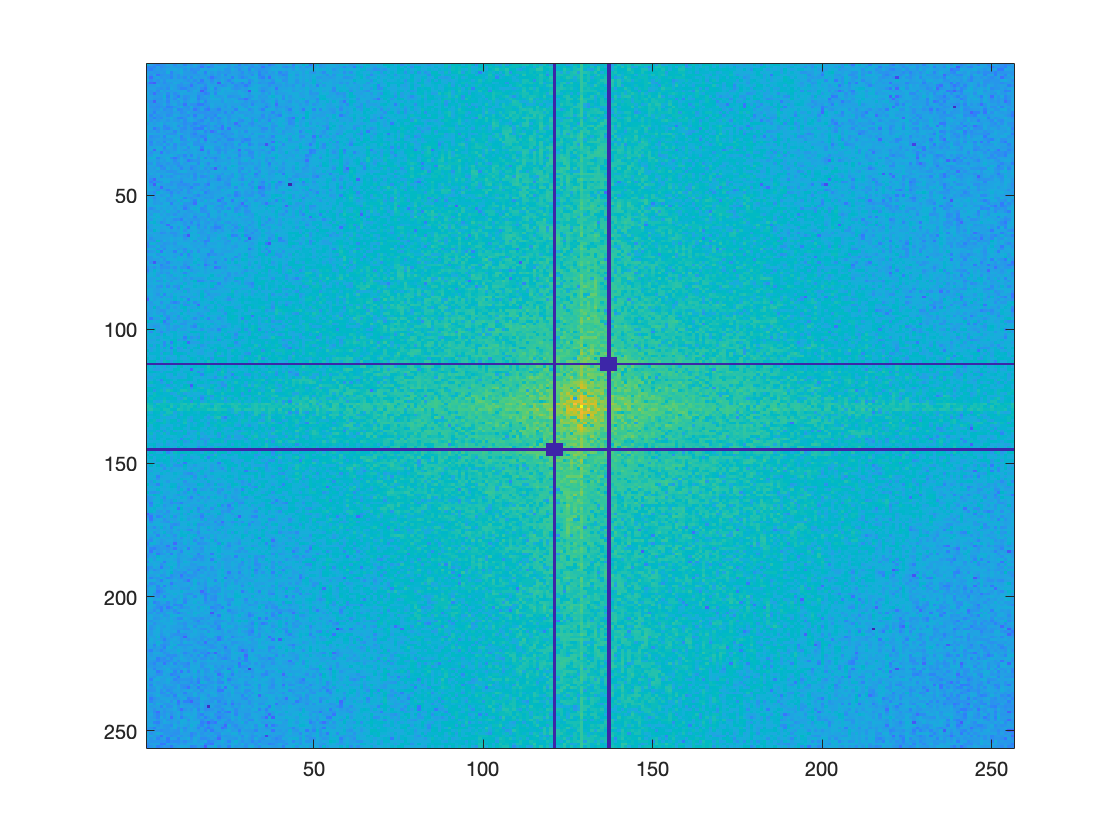
\includegraphics[width=0.7\textwidth]{fig26.png}
\end{figure}
\begin{figure}[H]
    \centering
    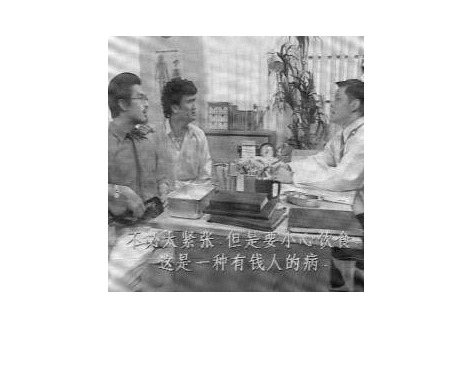
\includegraphics[width=0.7\textwidth]{fig27.png}
\end{figure}
\newpage
\subsection{Jailbreak}
Input:
\begin{minted}[bgcolor=cbg, fontsize=\footnotesize, mathescape]{octave}
% Display image
img = imread('primatecaged.jpg');
img = rgb2gray(img);
figure
imshow(img)

% Compute and display Fourier spectrum
ft = fft2(img);
S = abs(ft).^2 / length(img);
figure
imagesc(fftshift(log10(S)))

% Filter out frequencies corresponding to the fence
x1 = 11;
y1 = 252;
x2 = 247;
y2 = 6;
x3 = 21;
y3 = 248;
x4 = 237;
y4 = 10;
ft(y1-2 : y1+2, x1-2 : x1+2) = 0;
ft(y2-2 : y2+2, x2-2 : x2+2) = 0;
ft(y3-2 : y3+2, x3-2 : x3+2) = 0;
ft(y4-2 : y4+2, x4-2 : x4+2) = 0;
S = abs(ft).^2 / length(img);
figure
imagesc(log10(S))

% Display new image
img = uint8(ifft2(ft));
figure
imshow(img)
\end{minted}
\newpage
Output:
\begin{figure}[H]
    \centering
    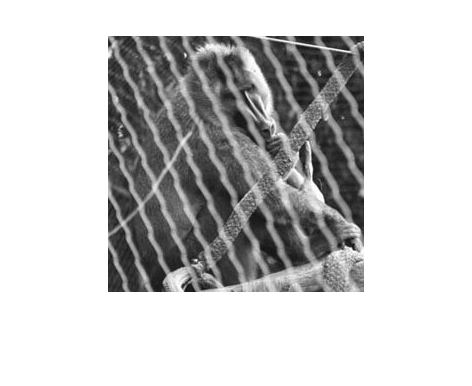
\includegraphics[width=0.7\textwidth]{fig28.png}
\end{figure}
\begin{figure}[H]
    \centering
    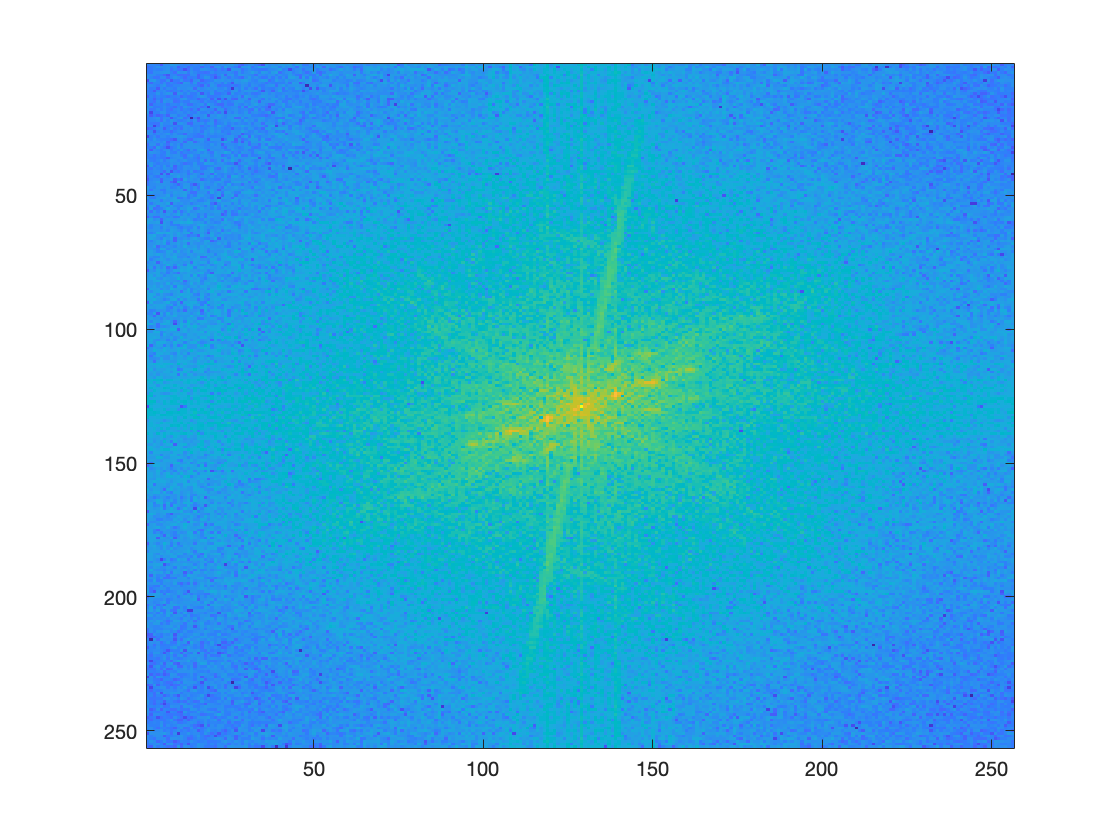
\includegraphics[width=0.7\textwidth]{fig29.png}
\end{figure}
\begin{figure}[H]
    \centering
    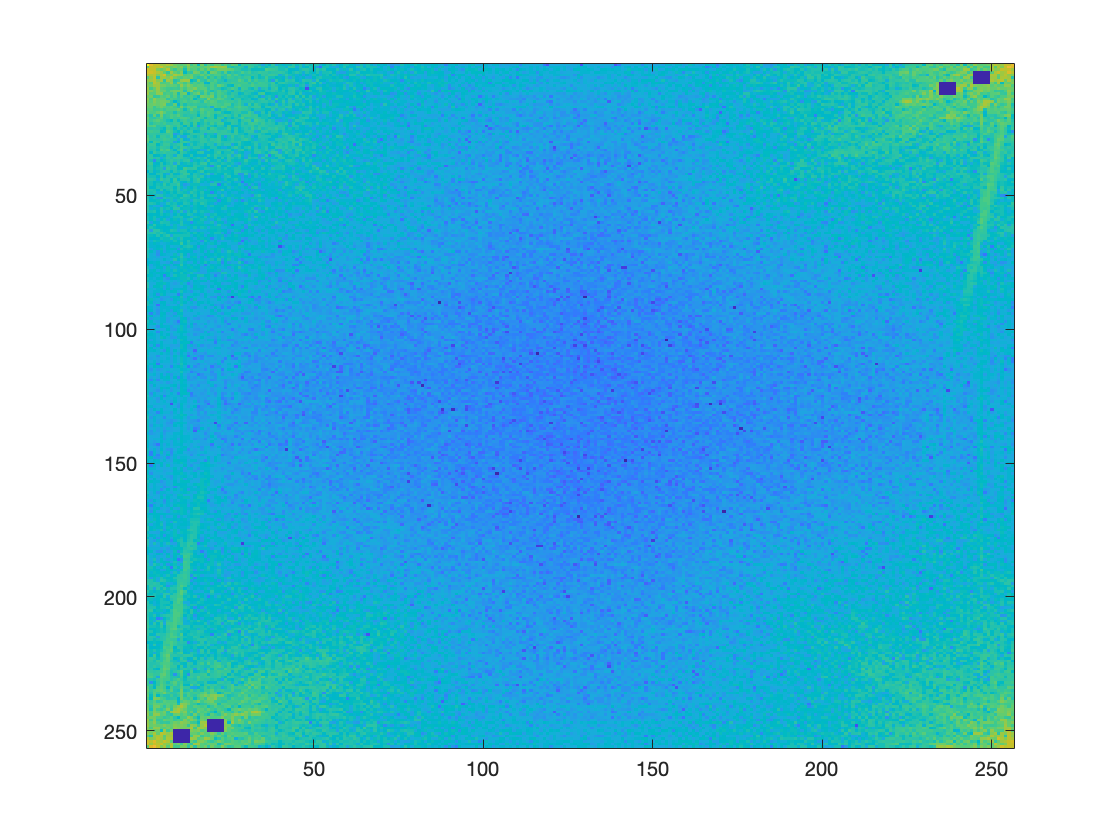
\includegraphics[width=0.7\textwidth]{fig30.png}
\end{figure}
\begin{figure}[H]
    \centering
    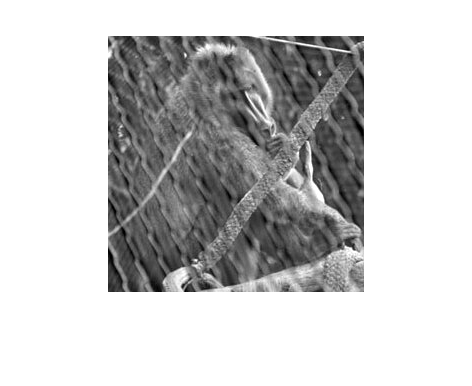
\includegraphics[width=0.7\textwidth]{fig31.png}
\end{figure}
~\\
As was to be expected, the fence is not gone but has rather been blurred a bit.
\newpage
\section{Undoing Perspective Distortion of Planar Surface}

\subsection{Load and display the image}
Input:
\begin{minted}[bgcolor=cbg, fontsize=\footnotesize, mathescape]{octave}
img = imread('book.jpg');
figure
imshow(img)
\end{minted}
Output:
\begin{figure}[H]
    \centering
    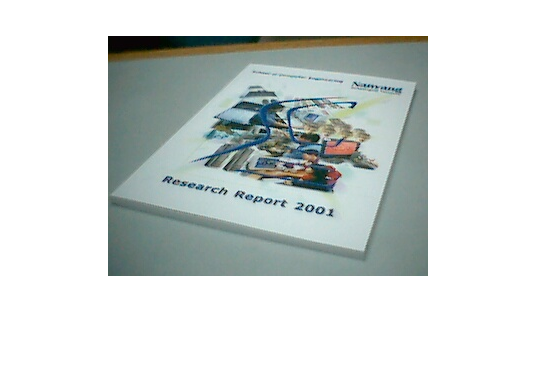
\includegraphics[width=0.7\textwidth]{fig32.png}
\end{figure}

\subsection{Specifying coordinates}
Input:
\begin{minted}[bgcolor=cbg, fontsize=\footnotesize, mathescape]{octave}
[X, Y] = ginput(4);
x = [0 210 210 0];
y = [0 0 297 297];
\end{minted}
\newpage
\subsection{Linear algebra intermezzo}
Input:
\begin{minted}[bgcolor=cbg, fontsize=\footnotesize, mathescape]{octave}
v = zeros(8, 1);
A = zeros(8, 8);
for i = 1:4
    A(2*i-1 : 2*i, :) = [X(i) Y(i) 1 0 0 0 -x(i)*X(i) -x(i)*Y(i);
                         0 0 0 X(i) Y(i) 1 -y(i)*X(i) -y(i)*Y(i)];
    v(2*i-1 : 2*i) = [x(i), y(i)];
end
u = A \ v;
U = reshape([u; 1], 3, 3)'   % Print U

% Verify U matrix
w = U * [X'; Y'; ones(1,4)];
w = w ./ (ones(3,1) * w(3,:))    % Print w
\end{minted}
Output:
\begin{minted}[bgcolor=cbg, fontsize=\footnotesize, mathescape]{text}
U =

    1.4539    1.5657 -253.2027
   -0.4499    3.7341  -39.7702
    0.0001    0.0054    1.0000


w =

   -0.0000  210.0000  210.0000   -0.0000
         0         0  297.0000  297.0000
    1.0000    1.0000    1.0000    1.0000
\end{minted}
The transformation returns the correct coordinates.

\subsection{Warping the image}
Input:
\begin{minted}[bgcolor=cbg, fontsize=\footnotesize, mathescape]{octave}
T = maketform('projective', U');
i2 = imtransform(img, T, 'XData', [0 210], 'YData', [0 297]);
\end{minted}
\newpage
\subsection{Displaying the result}
Input:
\begin{minted}[bgcolor=cbg, fontsize=\footnotesize, mathescape]{octave}
figure
imshow(i2)
\end{minted}
Output:
\begin{figure}[H]
    \centering
    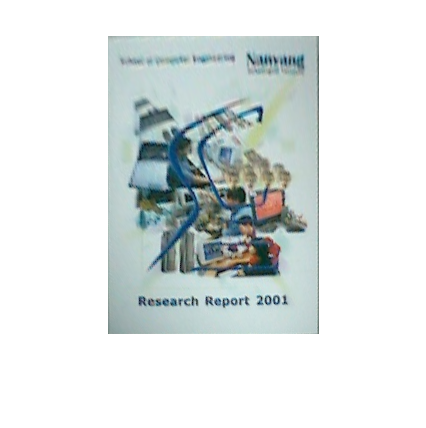
\includegraphics[width=0.7\textwidth]{fig33.png}
\end{figure}
~\\
The result is as expected; the distortion has completely been removed. The image is much sharper in the bottom-right corner, because that is where the target was nearest to the camera in the original image. The original image did already have a low resolution, making it impossible to accurately reproduce e.g. the text in the top-left corner, because the information was not present in the original image. The text ``Research Report 2001'' is also less sharp than before, which is due to the low resolution of the original image; the text was captured at an angle, which is represented in the pixels. Because the pixels have to stay rectangular and cannot be rotated, it is impossible to accurately undo this slant without an original image of higher resolution.

\end{document}